In addition to the fitting of the models to the Myeloma data, we also fitted the models to colon cancer data collected from \cite{Palmer1883,SEER}. This data was processed in the same way as the Myeloma data with the modification that all ages below 12 years were removed in this data set as oppose to removing all ages below 25 years in the Myeloma data set. At first, the model selection problem with the colon cancer data looks similar to the one with Myeloma cancer but reversed, as the fits of both models are really good but the PLM has a slightly better fit with $R_{\mathrm{adj}}=0.9953$ than the IM-II with $R_{\mathrm{adj}}=0.9921$ (Fig \ref{fig:colon}). However, when we performed Vuong's non-nested likelihood ratio test \cite{Vuong1989} on this time series, it turns out that these models are in fact distinguishable where the PLM fits the data better than the IM-II (Tab \ref{tab:fit_data}). Also, we performed a variance test in $R$ (Tab \ref{tab:variance_test}) where the conclusion is that the two models are indistinguishable in both the case of the Myeloma cancer \textit{and} the case of the colon cancer data. Thus, the variance test suggests that both are indistinguishable in contrast to Vuong's non-nested likelihood ratio test. Based on these two test we decided to work with the Myeloma data as both statistical tests suggest that the models are indistinguishable.  




\begin{figure}[htbp!]
  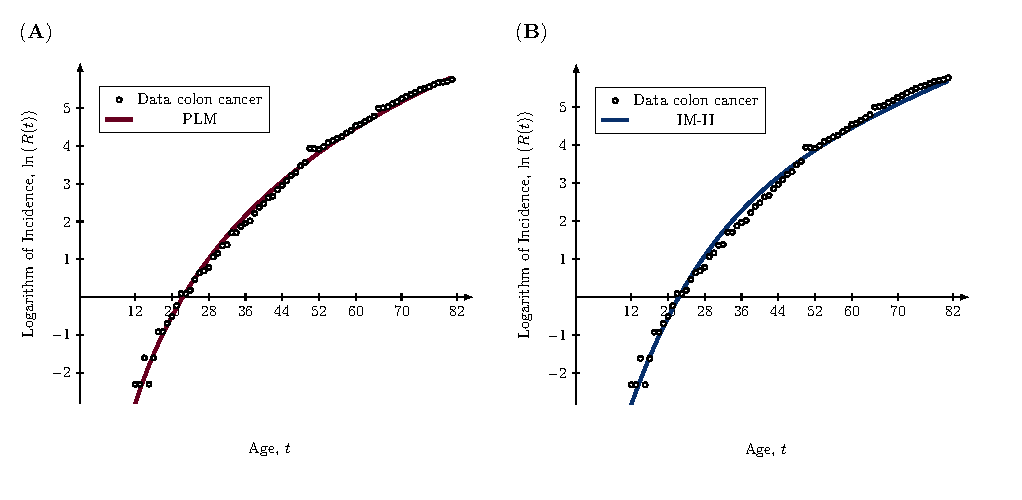
\includegraphics[width=\textwidth]{colon_cancer_fit}
  \caption[Both the PLM and the IM-II fit colon cancer data well]{\textit{Both the PLM and the IM-II fit colon cancer data well}. Two models are fitted to the processed time series consisting of the logarithms of the incidences of colon cancer for ages in the range $(12, 83)$ years which is illustrated in two cases. (\textbf{A}) The PLM with optimal parameters $(\ln(A),\gamma)=(-14.0715,4.5280)$ and fit $R_{\mathrm{adj}}=0.9953$. (\textbf{B}) The IM-II with optimal parameters $(\ln(A),\alpha,\tau )=(4.8731,0.044,58.3782)$ and fit $R_{\mathrm{adj}}=0.9921$.}
  \label{fig:colon}
\end{figure}





\begin{table}[htbp!]
\begin{center}
    \caption[The fit of the two candidate models to the colon cancer data]{\textit{The fit of the two candidate models to the colon cancer data}. The columns from left to right are: the name of the model, the function describing the solution curve, the optimal fit $R^2_{\mathrm{adj}}$ and the optimal parameters. In the symmetry based methodology for model selection, it is the parameter $A$ that is fitted to the transformed time series for both the PLM and the IM-II. The parameters $\gamma$ in the former case and the parameter $\tau$ in the latter case are fixed to their optimal values displayed in this table. The parameter $\alpha$ in the IM-II is held constant meaning that it is not estimated and its value is set to $\alpha=0.044$ \cite{Palmer1883}. The IM-II contains a ``double exponential'' for which we have chosen the notation ``$\exp(e^x)$''. To statistically test whether the fits of the two models are equal, we have performed Vuong's non-nested likelihood ratio test \cite{Vuong1989} where a $p$-value that is larger than $0.05$ means that the null hypothesis $H_0$ is likely to be true.}
    \begin{tabular}{||p{2.3cm}|c|p{1.5cm}|p{2.0cm}|p{4.0cm}||}
    \hline\hline
         & & & & \\
       \textit{Model}  & \textit{Curve} & \textit{Optimal fit, $R^{2}_{\mathrm{adj}}$} & \textit{Optimal parameters} & \textit{Non-nested likelihood ratio test}\\
         & & & & \\
        & & & & $H_0:$ Model fits are equal\\
         & & & & \\
      \hline\hline     
      & & & & \\
      Power law model & $R(t)=At^{\gamma}$ & $0.9953$ & $\ln\left(A\right)\approx-14.0715$ & $H_1$: the PLM fits better than the IM-II\\
      (PLM) & & & $\gamma\approx 4.5280$ & $p=2.19\cdot 10^{-5}$\\
      & & & &\\
      \hline
      & & & & \\
        & & & $\ln\left(A\right)\approx 4.8731$ & \\
    Immunological model & $R(t)=\dfrac{A}{\exp\left(e^{-\alpha(t-\tau)}\right)-1}$ & $0.9921$ & $\tau\approx 58.3782$ & $H_1$: the IM-II fits better than the PLM\\
      (IM-II) & & & $\alpha=0.044$ (Fixed) & $p=1$\\
      & & & & \\
      \hline\hline
    \end{tabular}
    \label{tab:fit_data}
\end{center}
\end{table}



\begin{table}[htbp!]
  \begin{center}
    \caption[The variance test suggests that both models are indistinguishable when fitted to two different data sets.]{\textit{The variance test indicate the both models are indistinguishable when fitted to two different data sets}.  A value of $p<0.05$ indicates that the null hypothesis $H_o$ is likely to be true while a value of $p>0.05$ indicates that the alternative hypothesis $H_1$ is true. }
    \begin{tabular}{||c|c||}
\hline\hline
      &  \\
      \textit{Data set} & \textit{Statistical hypotheses}\\
      & $H_0$: the PLM and the IM-II are indistinguishable \\
      & $H_1$: the PLM and the IM-II are distinguishable \\
      &  \\
      \hline\hline
      &  \\
      Myeloma cancer  & $p=0.00718$\\
      &  \\
      \hline
      &  \\
      Colon cancer & $p<2\cdot 10^{-16}$ \\
      &  \\
      \hline
      \hline\hline
      \end{tabular}
\label{tab:variance_test}
\end{center}
 \end{table}
